%\documentclass[12pt,a4paper, bibliography=totoc, listof=numbered, footexclude]{scrartcl}
\documentclass[12pt,a4paper, bibliography=totoc, listof=numbered, footexclude]{scrartcl}
\usepackage[utf8]{inputenc}		
\usepackage[T1]{fontenc}     % T1: Kodierung mit der Latex speichert, fontenc: Kodierung, wie er Tastatureingaben interpretiert beim Compilieren
\usepackage[british,UKenglish,USenglish,english,american]{babel}
\usepackage{amsmath}
\usepackage{amsfonts}
\usepackage{url}
\usepackage{amssymb}
\usepackage{graphicx}                         
\usepackage{float}
\usepackage{epstopdf}
\usepackage{caption}
\captionsetup{font=small}
\usepackage{tocloft}
\usepackage{fancyhdr}
\pagestyle{fancy}
\usepackage[]{acronym}
\newcommand{\acrounit}[1]{
  \acroextra{\makebox[18mm][l]{\si[]{#1}}}}
  \usepackage{siunitx}
  \renewcommand*{\bflabel}[1]{{\textsf{#1}\hfill}}
  
\begin{document}


 \title{Project 1: Information Transmission in Spiking Networks}
 \author{Oliver Eberle \ \  Malte Esders \ \ Tabea Kossen}
 \maketitle 
   \thispagestyle{empty}
 \newpage
 \section{Introduction}
 The mechanisms of information proceessing in the brain are one of the big questions in neuroscience. Classically, there are two main theories of how information is encoded via neural spiking - either by firing rate (frequency or rate coding) or by timing of occurence (temporal coding).\\
 Using  firing rate as a strategy to encode a stimulus ignores all of a spike's temporal information, since only the number of spikes per time interval count. On the one hand this limits the information capacity but on the other hand results in a robust method for coding in a noisy environment.\\
 However, computing firing rates over time windows takes time and capacitative resources and thus, the idea of temporal coding as a quicker and more efficient alternative attracted rising attention.\\
 Still, critics claim that ongoing background activity makes it hard to convey precise spike timings in a network.\footnote{R. 
 VanRullen, R. Guyonneau, S. J.  Thorpe, Spike times make sense, TRENDS in neuroscience, Vol. 28, No. 1, January 2005, \url{http://www.neuro.uoregon.edu/wehr/coursepapers/vanrullen-thorpe-2004.pdf}} This hypothesis was for example investigated looking at the  propagation of synchronous spike volleys through a multilayer feed-forward network. \footnote{M. Diesmann, M.-O. Gewaltig, A. Aertsen, Stable
 propagation of synchronous spiking in cortical neural networks. Nature
 402(2):529-532., 1999} It was shown that, in dependence of the number of input spikes and their temporal deviation, the network is able to preserve and produce synchronicity. In the following the possibility of synchronous spiking in a feed-forward network is examined.
 
  
 \section{Methods}
 \subsection{Leaky integrate and fire model}
 To model electric neural properties a conductance based leaky integrate and fire model was used:
 \begin{align}
 \tau_m\frac{dV}{dt}= (-V + E_m) + R_m (- I_{K^+} - I_{syn} + I_{noise})
 \end{align}
 
 Hereby, $\tau_m$ is the membrane time constant, $E_m$ the membrane potential, $R_m$ stands for the membrane resistance, which is multiplied by the $I_{K^+}$ potassium, $ I_{syn}$ synaptic and $I_{noise}$  noise currents, which pass through the membrane. \\
 If the membrane voltage $V$ reaches the threshold  $V_{thresh}$, $V$ is being resetted to the resting potential and a spike is counted. To model the decreased probabilty of another spike shortly after a previous one, an absolute refractory period was introduced, which deactivates incoming inputs from other neurons.\\
 Additonally, a relative refractory period was used, which describes the increase of the $K^+$ conductance after an action potential and the subsequent exponential decay:
  \begin{align}
  \frac{d g_K}{dt}=-\frac{g_K}{\tau_K} \\
  I_K=g_k(V-E_K)
  \end{align}
  Hereby, the $g_K$ conductance is manually increased after a postsnyaptic spike emerged.
  \begin{align}
   	g_K \rightarrow g_K + {\tilde{g}}_K
  \end{align}
  Background activity was modelled by an Ornstein-Uhlenbeck process (OUP), which is described by a stochastic differntial equation and is used to introduce background membrane potential activity.\footnote{V. Giorno, S.Spina, On the return process with refractoriness for a non-homogeneous Ornstein-Uhlenbeck neuronal model, Mathematical Biosciences, Vol. 12, No. 2, April 2014, \url{https://aimsciences.org/journals/pdfs.jsp?paperID=9176&mode=full}} Characteristic for the OUP is the so-called mean reversion, which expresses a non-constant drifting force towards the long-termn mean value.
  

   \begin{align}
   \  \frac{d I_{noise}}{dt}=\frac{{I_\mu}-I_{noise}}{\tau_{OUP}} {+ \sigma \eta}
   \end{align}
   
  \subsubsection*{Assumptions and parameters}
  In the model it is assumed that all neurons have the same properties, including an uniform number of synapses per neuron and equal strength for all synapses.
  Only excitatory neurons are implemented, assuming that the role of inhibitory neurons is included in the noise, helping to convey precise information via spike times.\\
  The noise values $I_{\mu}$ and $\sigma$ were adapted, so that it produces two spikes per second.
   Post-synaptic potentials were determined so that they would peak after 1.4 ms with a voltage of $0.11$ mV (compared to resting potential). 

  Used values for the mentioned parameters are as follows:
  
	\renewcommand{\baselinestretch}{0.1}\normalsize
   \begin{acronym}[LONGEST]
      % Allgemein:
      % Als Beispiele:
      \acro{Dt}[\ensuremath{\Delta t}]{ \ \ 0.1 ms \ \ \ \ \ \ \ \ \ \ Simulation time step }
	 \acro{restPot}[\ensuremath{E_K}]{ \acrounit{-77 mV} \ \ \  \ \ \ \ $K^+$ equilibiurm potential }
	 \acro{Vtresh}[\ensuremath{V_{tresh}}]{ \acrounit{-55 mV} \ \ \  \ \ \ \ Spiking threshold }		
     \acro{eqPot}[\ensuremath{E_m}]{ \acrounit{-70 mV} \ \ \  \ \ \ \ Membrane resting potential}
     \acro{gconducadd}[${\tilde{g}}_K$]{ \ \acrounit{5 nS}   \ \  \  \ \ Additive K-conductance} 
     \acro{MemRes}[$R_m$]{ \ \acrounit{10$^7$ \ohm}   \ \  \  \ \ Membrane resistance}
     \acro{tausyn}[\ensuremath{\tau_{syn} }]{ \ \ 0.335 ms \ \  \ \ \ \ \ Synaptic time constant }
     \acro{tauOUP}[\ensuremath{\tau_{OUP} }]{ \ \ 5 ms \ \ \ \ \ \  \   \ \ \ \ \ Noise time constant }
     \acro{sig}[\ensuremath{\sigma }]{ \ \ 10$^{-7}$ \ \ \  \ \ \ \ \ \ \ \ \ Standard deviatoin of noise current }
      \acro{Imu}[\ensuremath{I_{\mu}} ]{ \ \  0.886 pA \ \  \ \ \   \ Mean noise current  }
              

    \end{acronym}
   \renewcommand{\baselinestretch}{1.0}\normalsize
  
  \subsection{Implementation}
  The network is implemented using an object-oriented approach in Python 2.7. The model is working via three interactive classes: a model neuron class, a synapse class and a noise class. In order to be able to efficiently control the behavior of the model, most functionality is $hidden$ within the classes, so that as litte as possible code is needed to create new neuronal networks.\\
  When a neuron object is created, it automatically creates a noise object from which it will draw its $personalised$ noise. This is necessary because the noise is not simple gaussian noise, but follows the Ornstein-Uhlenbeck process (see Fig. \ref{fig:noise} below). Once created, the neuron objects need to be assigned other neurons that they are projecting onto. When this is done, the neurons will create as many synapse objects as needed to simulate synaptic transmision. Every synapse object has its own timing and will be activated by its host neuron after the corresponding presynaptic neuron fires.\\
  In the network, 1000 neurons are created, who are separated into 10 groups of equal size. The first group projects onto the second group, all neurons from the first group have a synapse with all neurons from the second, and so on, which results in 90.000 synapses total (not 100.000 since the last group does not project to another group. This results in a fully connected feed forward network (synfire chain).
    	\begin{figure}[H]
  
    	  		\centering
    	  		  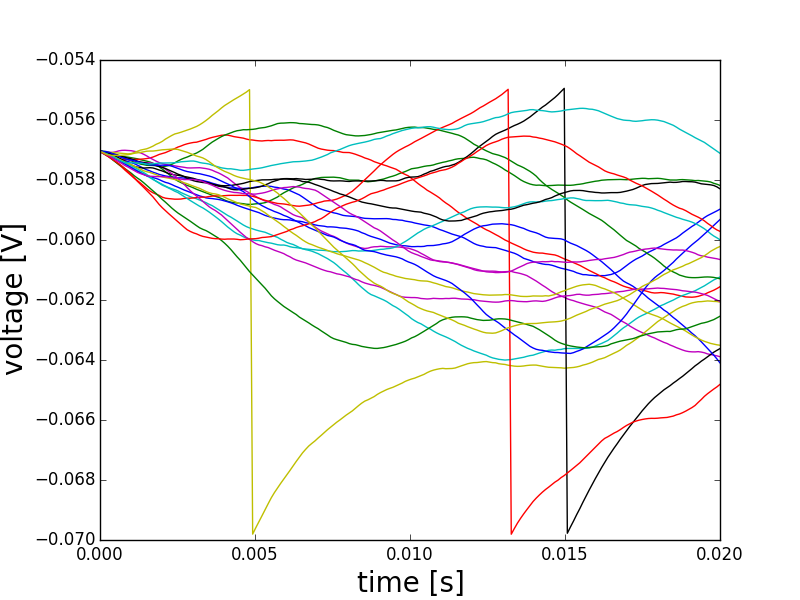
\includegraphics[width=0.8\linewidth]{./Plots/Our_Plots/noise_grosse_schrift}
  
    
    			  \caption{ Voltage time course in dependence of Ornstein-Uhlenbeck current. }
      	  		  \label{fig:noise}
   
    	    	
    	    	\end{figure}
  

  
  \section{Results}

  When applying 40 artifical spikes to the first group of 100 neurons, synchronization can be observed (reference Fig. \ref{fig:voltageplot_synchronization} and \ref{fig:rasterplot}). Figure  \ref{fig:voltageplot_synchronization} shows the voltage trace of each neuron over time. At about 5ms (varying standard deviation) the first group receives the input spikes. This leads to a synchronization of all 10 groups. This is also shown in the raster plot (\ref{fig:rasterplot}). Here only the spikes are indicated by a line for each of the 1000 neurons.\\
  When applying only 30 artifical spikes to the first group, synchronization does not happen anymore (see Fig. \ref{fig:asynchronization_rasterplot}). The first groups are still firing more or less simultaneously but then synchrony slowly fades out.\\  
  The simulation was repeated several times with differing number of input spikes and differing standard deviation of spike onset (see Fig.\ref{fig:Phase_plane}). For each of the 13 startvalues, the simulation was done 100 times. The arrows represent the average over those trials for each starting point. In each group the standard deviation for the spikes was calculated, so that every arrow in the plot stands for one group. The arrows converge either to the top left or to the bottom right.
  
  \begin{figure}[H]
  \centering
  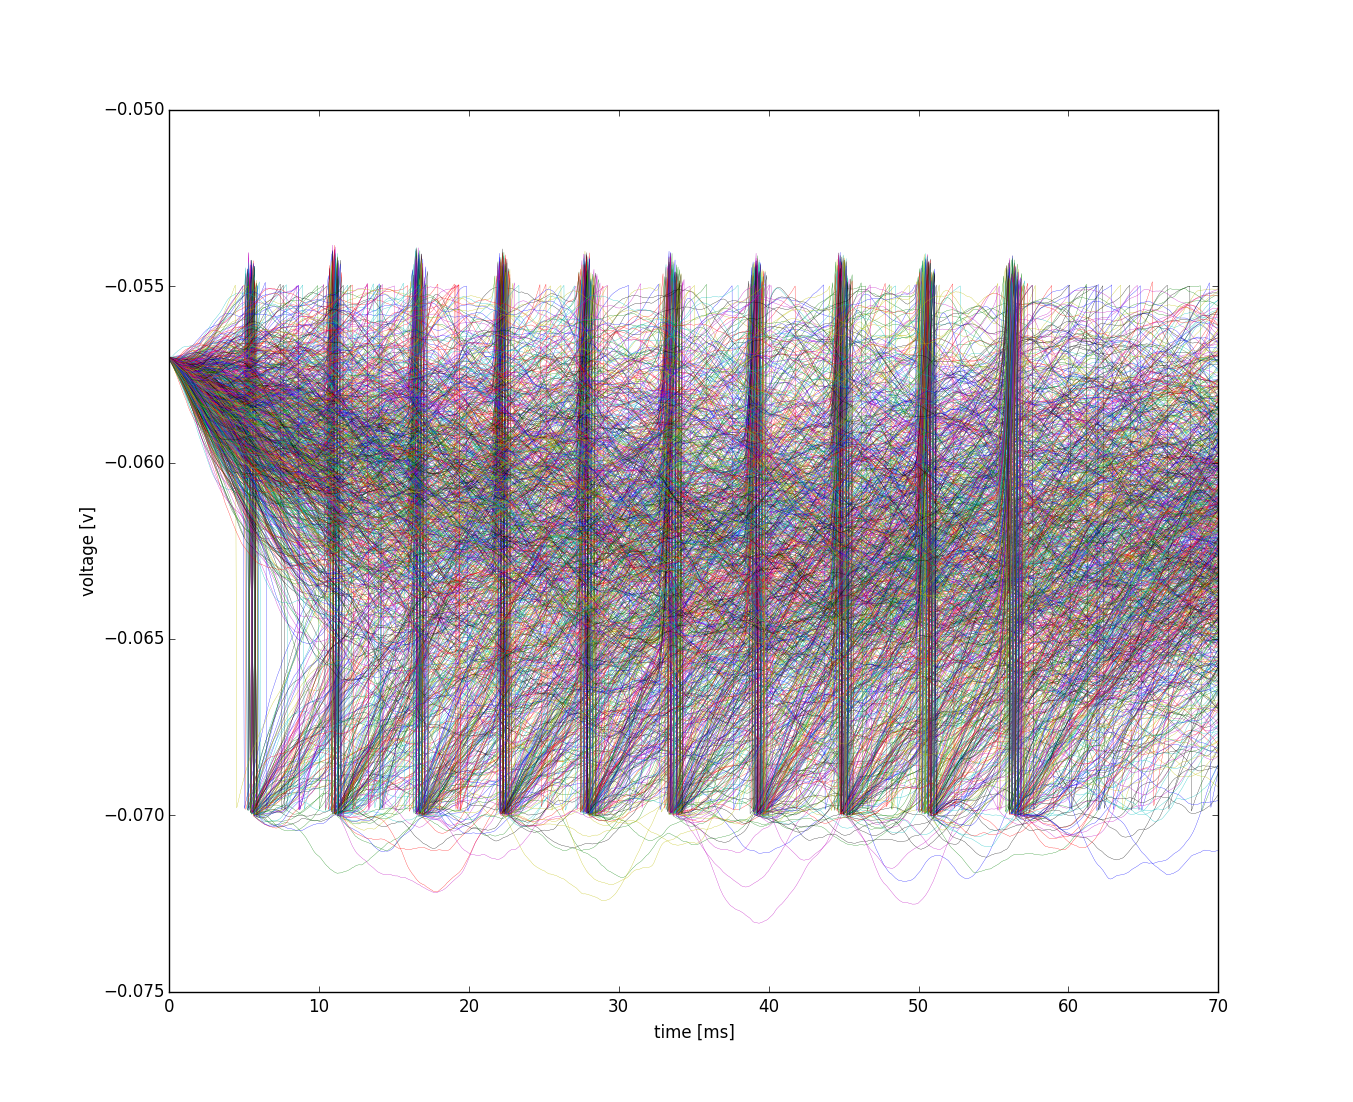
\includegraphics[width=0.9\linewidth]{./Plots/Our_Plots/voltageplot}
  \caption{Voltage traces of all 100 neurons in all of the 10 groups. Clearly visible are the spiking ensembles of the groups and a moderate synchronization process throughout the network. After reaching the threshold at $V_{thresh}=-54.0 mV$ the voltage is resetted to the resting potential $V_{rest}=-70.0 mV$. }
  \label{fig:voltageplot_synchronization}
  \end{figure}



	\begin{figure}[H]
	    	\begin{minipage}[hbt]{8.2 cm}
	  		\centering
	  		 
	  		  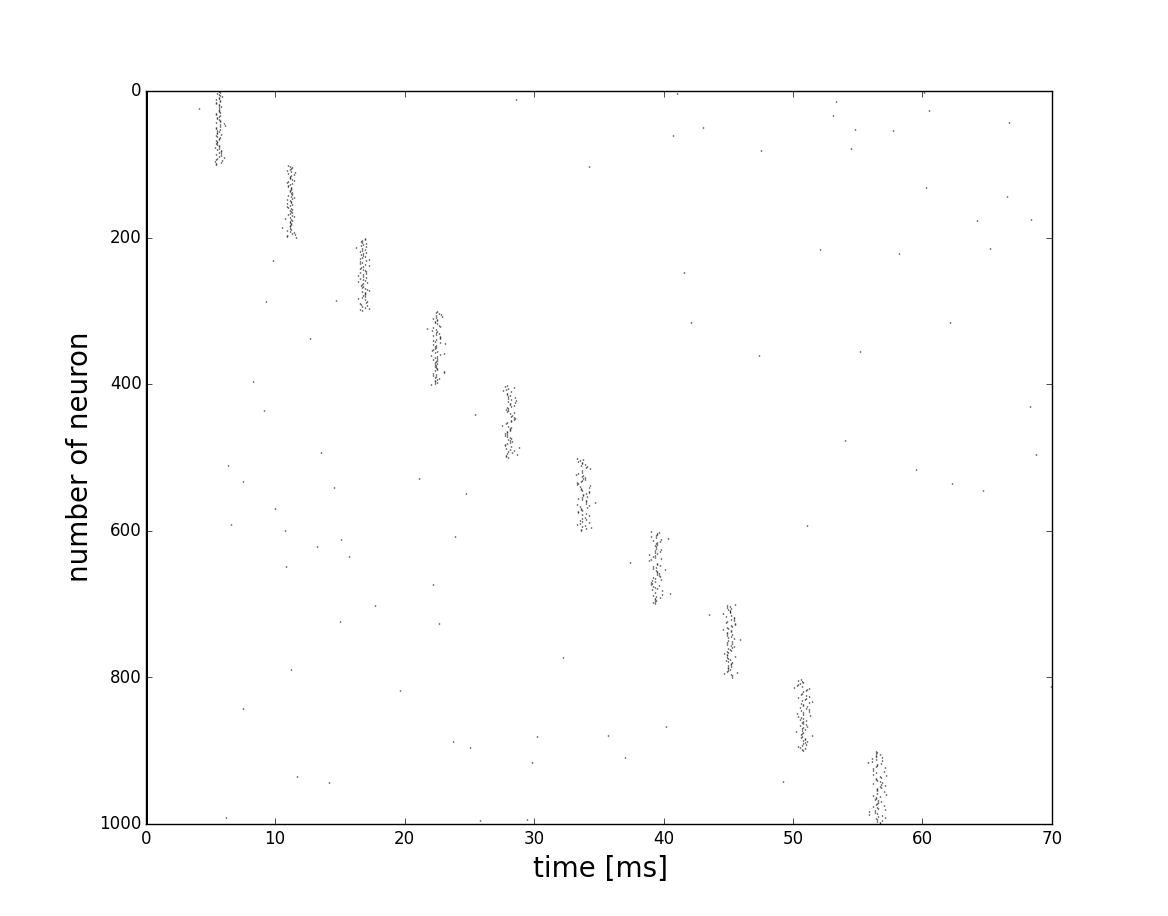
\includegraphics[width=1.0\linewidth]{./Plots/Our_Plots/rasterplot_grosse_schrift}
	  		  \caption{Synchronization}
	  		  \label{fig:rasterplot}
	    		
	    	\end{minipage}
  	    	\hfill
	    	\begin{minipage}[hbt]{8.2 cm}

	    \centering
	    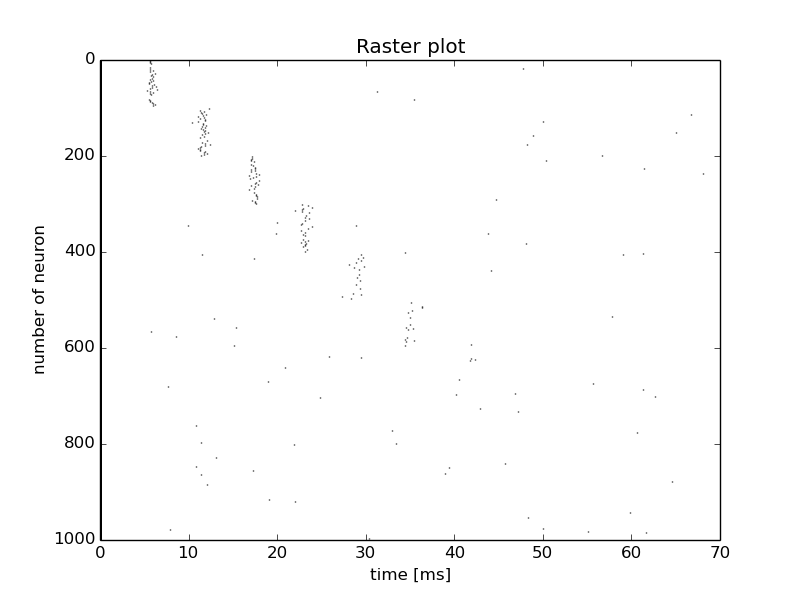
\includegraphics[width=1.0\linewidth]{./Plots/Our_Plots/asynchronization_rasterplot}
	    \caption{Asynchronization}
	    \label{fig:asynchronization_rasterplot}
	    	\end{minipage}
	    	\end{figure}
	  \begin{figure}
	\centering
	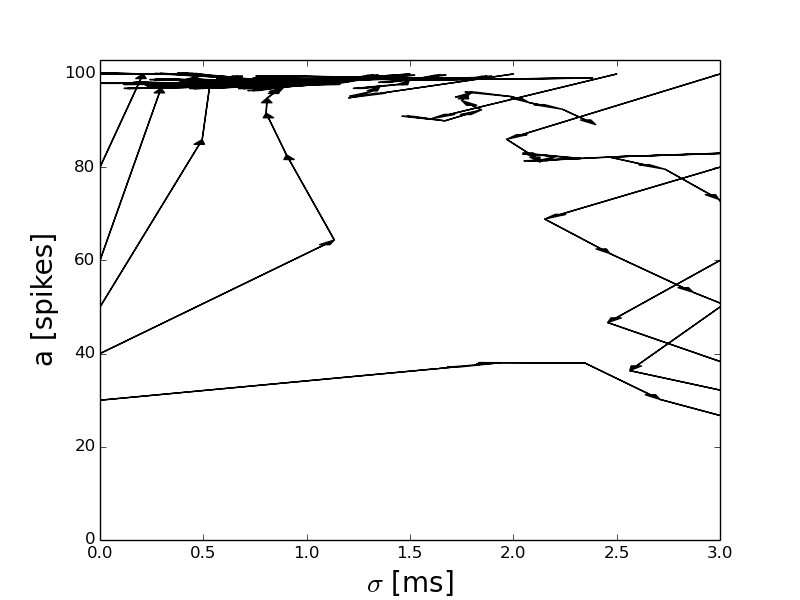
\includegraphics[width=0.92\linewidth]{./Plots/Our_Plots/Phase_plane}
	\caption{Visualized is the relationship between input spikes and standard deviaton. Every arrow represents one group and was obtained by averaging over multiple simulations. In the left upper corner the fixed point is identifiable.}
	\label{fig:Phase_plane}
	\end{figure}


  \section{Discussion}
  The purpose of this study was to find out whether spiking volleys can propagate through the brain despite considerable background noise. Since this study is a replication of the study by Diesmann et al. (1999), it was desirable to use exactly the same parameters. In practice this proved difficult, because the original paper did not specify all parameters to the necessary precision (e. g., the exact amount of background noise, or the parameters of the relative refractoriness modeled by K-conductances). An effort has been made to infer missing parameters, mainly by referring to plots of voltages of the neurons over time. With the help of these plots, parameters were chosen so that the voltage lines resembled voltage plots of real neurons.\\
  Throughout the project, the exact characteristics of background noise proved to be extremely important. Simulation results changed dramatically with extremely minor variations of the background noise paramters. In order to have realistic background noise, it was attempted to make its effect on neuronal voltage behavior non deterministic, that is, two neurons starting off at same voltage values and receiving background noise from the same algorithm could show very different behavior. Overall, it was accomplished to get reasonable-looking plots, but the parameters were still very different from the original paper. For this reason the results in the current simulation were slightly different, but qualitatively, earlier findings could be replicated. It could be shown that spike propagation can either synchronize or desynchronize across spike volleys, depending on spike number and spread characteristics. Group-firing patterns with low standard deviation and high spike count have a high chance to lead to synchronized firing in the next neuron group.\\
  A decrease in the amount of spikes in a group, or an increase in the spread of the spikes (or both) lead to a smaller probability of synchronized firng in the next group. In the  basin of attraction exists an attractor that many spike volleys will converge to, given that they are within the confines of the separatrix. When this is not the case, the system will converge to very few (random) spikes that are insufficient to induce firing in the next neuron group. This finding supports the theory that neurons can convey information not only by firing rate but also by specific spike timing. 
  
  \section{Conclusion}
  
  The main conclusion of this project is that information processing via spike timing is indeed possible in spite of the background noise. The noise does not necessarily interfere with the synchronization and even precise synchronous firing is feasible. This allows for an increased information capacity compared to frequency-coded information processing.
  
  For this network which carries information by precise spike timing a relatively large group of neurons is needed. However, neurons can participate in several volleys simultaneously and the network only needs to be locally feedforward.
 

\end{document}